\documentclass[12pt]{article}
\usepackage[a0paper]{geometry}
\usepackage[svgnames, dvipsnames, usenames]{xcolor}
\usepackage{lipsum}
\usepackage{lmodern}
\usepackage{enumerate}
\usepackage{adjustbox}
\usepackage[poster]{tcolorbox}
\tcbuselibrary{minted}
\pagestyle{empty}

% math mode package %
\usepackage{amsfonts}
\usepackage{amsmath}
\usepackage{mathtools}
\usepackage{amssymb}

\usepackage{tikz}
\usepackage{pgfplots}
\pgfplotsset{compat=newest}
\usetikzlibrary{arrows,angles,quotes}
\usepackage{graphicx}
\graphicspath{{.}}
\usepackage{caption}
\usepackage{subcaption}

\definecolor{Bblack}{HTML}{00004d}
\definecolor{maincolor}{HTML}{3BB9FF}
\begin{document}
\begin{tcbposter}[
    coverage = {
        spread,
        interior style={top color=maincolor!10!white,bottom color=maincolor!90!white},
        % watermark text={\LaTeX\ Poster},
        % watermark color=white,
        % enhanced,
        % frame hidden,
        boxsep=0.75cm,
        % boxrule=1cm,
        % top=4mm,
        % bottom=4mm,
        % left=4mm,
        % right=4mm,
        % toptitle=2mm,
        % bottomtitle=2mm,
        % colback=white
    },
    poster={showframe=false,
    columns=3,rows=5,spacing=6mm},
    boxes={
      enhanced standard jigsaw,
      sharp corners=northwest,
      arc=7.5mm,
      boxrule=1mm,
      colback=white,
      opacityback=0.75,
      colframe=maincolor!80!black,
      title style={left color=Bblack,right color=maincolor!80!black},
      fonttitle=\bfseries\Large\scshape,
      % halign=center,
      % valign=center
    },
    fontsize = 28pt
]
%%% Header box %%%
\posterbox[blankest,
    % interior engine=path,
    height=7.5cm,
    halign=left,
    valign=center,
    fontupper=\bfseries\large,
    % colupper=red!25!black,
    underlay={
    % \node[right,inner sep=0pt,outer sep=0pt] at (frame.west) {\includegraphics[height=3cm,width=3cm]{Mahidollogo.png}};
    \node[left,inner sep=0pt,outer sep=0pt] at (frame.east) {\includegraphics[height=20cm,keepaspectratio]{SCEN_1.png}};
    },
]
{name=title,column=1,span=3,below=top}{
    \resizebox{60cm}{!}{\color{maincolor!40!black}\sffamily\textbf{Orthogonal Equipartitions of 3-color Points in the Plane}}\\[1cm]
    % {\Huge\textbf{Orthogonal Equipartitions of 3-color Points in the Plane}}\\[1cm]
    % {\fontsize{66}{72}\textbf{Orthogonal Equipartitions of 3-color Points in the Plane}}\\[1cm]
    \large\underline{Krittapas Ngammmuengman}$^1$, Tirasan Khandhawit$^{1,}$*\\[5mm]
    % {Krittapas Ngammmuengman, {\mdseries Tirasan Khandhawit}}\\[5mm]
    {$^1$Department of Mathematics, Faculty of Science, Mahidol University, Bangkok, Thailand}
    \\[5mm]
    {*\texttt{tirasan.kha@mahidol.edu}}
    
    % \small{\texttt{krittapas.nga@student.mahidol.edu} \quad Department of Mathematics, Faculty of Science, Mahidol University}
}

%%%% Poster Tutorial 3,6 %%%%
\posterbox[adjusted title=References]{name=references,column=1,span=2,above=bottom}{
\begin{enumerate}[{[1]}]
\item\label{litA} S. Bereg, Orthogonal Equipartition, \textit{Computational Geometry} \textbf{42}, 305-314. (2009).
\item\label{litB} M. Uno, T. Kawano, M. Kano, Bisections of Two Sets of Points in the Plane Lattice, \textbf{Graphs and Combinatorics }\textbf{E92-A} (2009)
\item\label{litC} A. Kaneko, M. Kano, Balanced partitions of two sets of points in the plane, \textit{Comput. Geom. Theory Appl. }\textbf{13} (1999)
\end{enumerate}
}

\posterbox[adjusted title=Abstract]{name=abstract, column=1,span=2,below=title}{
\hspace{1\baselineskip} Orthogonal equipartition is a problem of subdividing the plane to regions containing equal numbers of points using only vertical and horizontal lines. Previously, Sergey Bereg proved that an equipartition of a set of 2-color points into two regions needs at most 1 horizontal and 1 vertical segments. We will be interested in a set of 3-color points. We give an algorithm to find an equipartition into two regions with at most 3 vertical and 2 horizontal segments. We also find examples that cannot be equipartitioned with less than 5 segments.\\[1cm]
\textbf{Keywords:} Equitable subdivision, Orthogonal partition, Colored point sets
}
    
\posterbox[adjusted title=Objective]{name=objective,column=1,span=1,below=abstract}{
    \hspace{1\baselineskip} Minimizing the number of line segments of orthogonal equipartition of 3-color points in general position in the plane.}
\posterbox[adjusted title=Definitions]{name=definition,column=1,span=1,below=objective}{
    \hspace{1\baselineskip} 
    Let $A$ be a set of points in the plane. The points in set $A$ are lying in \textbf{general position} if no three points lie on the same line. In other words, any three points can make a triangle.
\begin{figure}[H]
\centering
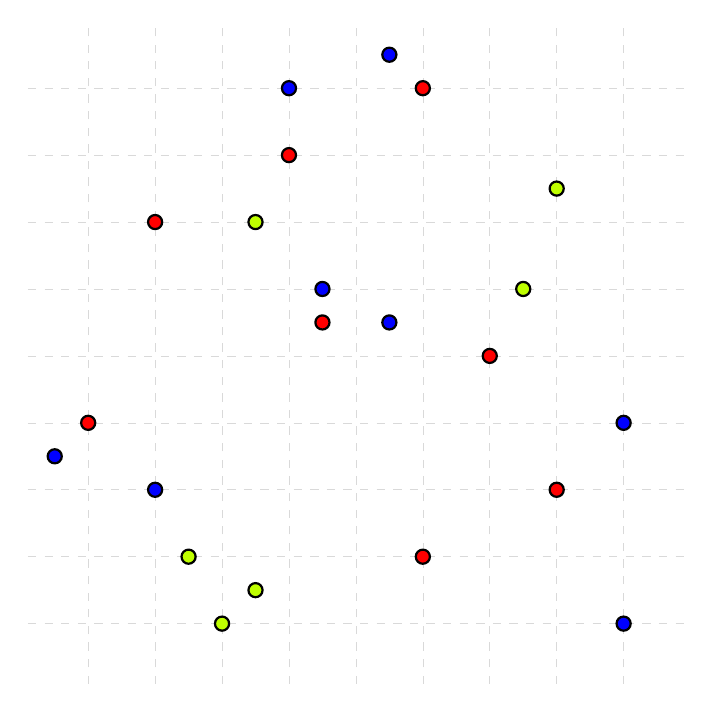
\begin{tikzpicture}[thick, scale=0.85]
%%%%% Axis %%%%%
\draw[help lines, color=gray!30, dashed] (-4.9,-4.9) grid (4.9,4.9);
% \draw[->,ultra thick] (-6,-5)--(5,-5) ;
% \draw[->,ultra thick] (-5,-6)--(-5,5) ;
%%%%% Point %%%%%
\draw[fill=lime,draw=black] (2.5,1) circle (3pt);
\draw[fill=lime,draw=black] (-2,-4) circle (3pt);
\draw[fill=lime,draw=black] (3,2.5) circle (3pt);
\draw[fill=lime,draw=black] (-2.5,-3) circle (3pt);
\draw[fill=lime,draw=black] (-1.5,2) circle (3pt);
\draw[fill=lime,draw=black] (-1.5,-3.5) circle (3pt);

\draw[fill=red,draw=black] (-1,3) circle (3pt);
\draw[fill=red,draw=black] (1,-3) circle (3pt);
\draw[fill=red,draw=black] (-3,2) circle (3pt);
\draw[fill=red,draw=black] (2,0) circle (3pt);
\draw[fill=red,draw=black] (-0.5,0.5) circle (3pt);
\draw[fill=red,draw=black] (1,4) circle (3pt);
\draw[fill=red,draw=black] (-4,-1) circle (3pt);
\draw[fill=red,draw=black] (3,-2) circle (3pt);

\draw[fill=blue,draw=black] (0.5,4.5) circle (3pt);
\draw[fill=blue,draw=black] (-0.5,1) circle (3pt);
\draw[fill=blue,draw=black] (-4.5,-1.5) circle (3pt);
\draw[fill=blue,draw=black] (4,-4) circle (3pt);
\draw[fill=blue,draw=black] (0.5,0.5) circle (3pt);
\draw[fill=blue,draw=black] (-1,4) circle (3pt);
\draw[fill=blue,draw=black] (-3,-2) circle (3pt);
\draw[fill=blue,draw=black] (4,-1) circle (3pt);
\end{tikzpicture}
\end{figure}
\hspace{1\baselineskip}The \textbf{orthogonal partition} consists of vertical line segments and horizontal line segments such that the intersection of any two segment is either an empty set or a vertex of two segments.
\begin{figure}[H]
\centering
\begin{subfigure}{0.32\textwidth}
\centering
\begin{tikzpicture}[thick, scale=0.85]
%%%%% Axis %%%%%
\draw[help lines, color=gray!30, dashed] (-4.9,-4.9) grid (4.9,4.9);
% \draw[->,ultra thick] (-6,-5)--(5,-5) ;
% \draw[->,ultra thick] (-5,-6)--(-5,5) ;
\draw[densely dashed,color=red,line width=1pt,opacity=1](-2,-5)--(-2,0)--(2,0)--(2,5);
% \foreach \i in {-5,-4.5,...,-3,-2.5}{
% \draw[densely dashed,color=blue,line width=0.5pt,opacity=1] (\i,-5)--(\i,5);
% }
% \foreach \i in {-2,-1.5,...,1,1.5}{
% \draw[densely dashed,color=blue,line width=0.5pt,opacity=1] (\i,0)--(\i,5);
% }
% \node at (-5.5,0) {$\color{red!80!black}i_1$};
% \node at (-2,-5.5) {$\color{red!80!black}j_1$};
% \node at (2,-5.5) {$j$};
\end{tikzpicture}
\end{subfigure}
\begin{subfigure}{0.32\textwidth}
\centering
\begin{tikzpicture}[thick, scale=0.85]
%%%%% Axis %%%%%
\draw[help lines, color=gray!30, dashed] (-4.9,-4.9) grid (4.9,4.9);
% \draw[->,ultra thick] (-6,-5)--(5,-5) ;
% \draw[->,ultra thick] (-5,-6)--(-5,5) ;
\draw[densely dashed,color=red,line width=1pt,opacity=1] (2,-5)--(2,-2)--(-2,-2)--(-2,2)--(2,2)--(2,5);
% \node at (-5.5,-2) {$i_1$};
% \node at (-5.5,2) {$\color{red!80!black}i_2$};
% \node at (-2,-5.5) {$j_1$};
% \node at (2,-5.5) {$j$};
% \foreach \i in {-5,-4.5,...,-3,-2.5}{
% \draw[densely dashed,color=blue,line width=0.5pt,opacity=1] (\i,-5)--(\i,5);
% }
% \foreach \i in {-2,-1.5,...,1,1.5}{
% \draw[densely dashed,color=blue,line width=0.5pt,opacity=1] (\i,-5)--(\i,-2);
% \draw[densely dashed,color=blue,line width=0.5pt,opacity=1] (\i,2)--(\i,5);
% }
\end{tikzpicture}
\end{subfigure}
\begin{subfigure}{0.32\textwidth}
\centering
\begin{tikzpicture}[thick, scale=0.85]
%%%%% Axis %%%%%
\draw[help lines, color=gray!30, dashed] (-4.9,-4.9) grid (4.9,4.9);
% \draw[->,ultra thick] (-6,-5)--(5,-5) ;
% \draw[->,ultra thick] (-5,-6)--(-5,5) ;
\draw[densely dashed,color=red,line width=1pt,opacity=1] (3,-5)--(3,-2)--(1,-2)--(1,-3)--(-2,-3)--(-2,-1)--(0,-1)--(0,1)--(-3,1)--(-3,2)--(2,2)--(2,5);
% \node at (-5.5,-2) {$i_1$};
% \node at (-5.5,2) {$\color{red!80!black}i_2$};
% \node at (-2,-5.5) {$j_1$};
% \node at (2,-5.5) {$j$};
% \foreach \i in {-5,-4.5,...,-3,-2.5}{
% \draw[densely dashed,color=blue,line width=0.5pt,opacity=1] (\i,-5)--(\i,5);
% }
% \foreach \i in {-2,-1.5,...,1,1.5}{
% \draw[densely dashed,color=blue,line width=0.5pt,opacity=1] (\i,-5)--(\i,-2);
% \draw[densely dashed,color=blue,line width=0.5pt,opacity=1] (\i,2)--(\i,5);
% }
\end{tikzpicture}
\end{subfigure}
\end{figure}
\hspace{1\baselineskip} Let $a$ and $b$ be positive integers. A partition of the plane into two regions $A$ and $B$ is called \textbf{$\boldsymbol{(a,\,b)-}$balanced with respect to a measure $\boldsymbol{\lambda}$} if $$\lambda(A)=\dfrac{a}{(a+b)} \text{ and } \lambda(B)=\dfrac{b}{(a+b)}$$ and called \textbf{$\boldsymbol{(a,\,b)-}$balanced} if it is $(a,\,b)-$balanced with respect to both measure $\lambda$ and $\mu$. We say that $(a,\,b)-$balanced partition is \textbf{equitable} if $a=b$.
}
\posterbox[adjusted title=Notations]{name=notation, column=1, below=definition}{
\hspace{1\baselineskip} 
Let $A$ is a set of $k-$color points in general position on lattice $\mathbb{Z}^2$ with length $n\times n$, where $n>1$ and $k>2$ be integers.\\
Defined $a_{ij}$ is a $k\times 1$-dimensional matrix of the number of points of each color over $y=i$ from $x=0$ to $x=j$.
\begin{figure}[H]
    \centering
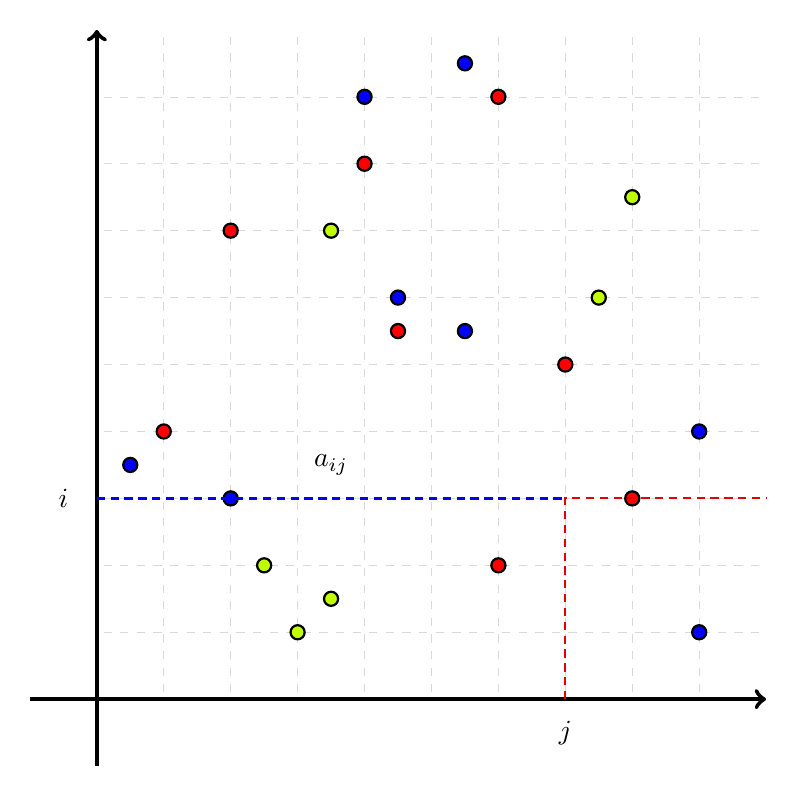
\begin{tikzpicture}[thick, scale=0.85]
%%%%% Axis %%%%%
\draw[help lines, color=gray!30, dashed] (-4.9,-4.9) grid (4.9,4.9);
\draw[->,ultra thick] (-6,-5)--(5,-5) ;
\draw[->,ultra thick] (-5,-6)--(-5,5) ;
%%%%% Point %%%%%
\draw[fill=lime,draw=black] (2.5,1) circle (3pt);
\draw[fill=lime,draw=black] (-2,-4) circle (3pt);
\draw[fill=lime,draw=black] (3,2.5) circle (3pt);
\draw[fill=lime,draw=black] (-2.5,-3) circle (3pt);
\draw[fill=lime,draw=black] (-1.5,2) circle (3pt);
\draw[fill=lime,draw=black] (-1.5,-3.5) circle (3pt);

\draw[fill=red,draw=black] (-1,3) circle (3pt);
\draw[fill=red,draw=black] (1,-3) circle (3pt);
\draw[fill=red,draw=black] (-3,2) circle (3pt);
\draw[fill=red,draw=black] (2,0) circle (3pt);
\draw[fill=red,draw=black] (-0.5,0.5) circle (3pt);
\draw[fill=red,draw=black] (1,4) circle (3pt);
\draw[fill=red,draw=black] (-4,-1) circle (3pt);
\draw[fill=red,draw=black] (3,-2) circle (3pt);

\draw[fill=blue,draw=black] (0.5,4.5) circle (3pt);
\draw[fill=blue,draw=black] (-0.5,1) circle (3pt);
\draw[fill=blue,draw=black] (-4.5,-1.5) circle (3pt);
\draw[fill=blue,draw=black] (4,-4) circle (3pt);
\draw[fill=blue,draw=black] (0.5,0.5) circle (3pt);
\draw[fill=blue,draw=black] (-1,4) circle (3pt);
\draw[fill=blue,draw=black] (-3,-2) circle (3pt);
\draw[fill=blue,draw=black] (4,-1) circle (3pt);
\draw[densely dashed,color=blue,line width=1pt,opacity=1] (-5,-2)--(2,-2);
\draw[densely dashed,color=red!90!black,line width=0.75pt,opacity=1] (2,-5)--(2,-2)--(5,-2);
\node at (-5.5,-2) {$i$};
\node at (2,-5.5) {$j$};
\node at (-1.5,-1.5) {$a_{ij}$};
\end{tikzpicture}
\end{figure}
\hspace{1\baselineskip} Defined $S_j$ by $k\times 1$-dimensional matrix of the number of points of each color on the left side of a line $x=j$, that is $S_j=\displaystyle\sum_{i=1}^na_{ij}$.
\begin{figure}[H]
    \centering
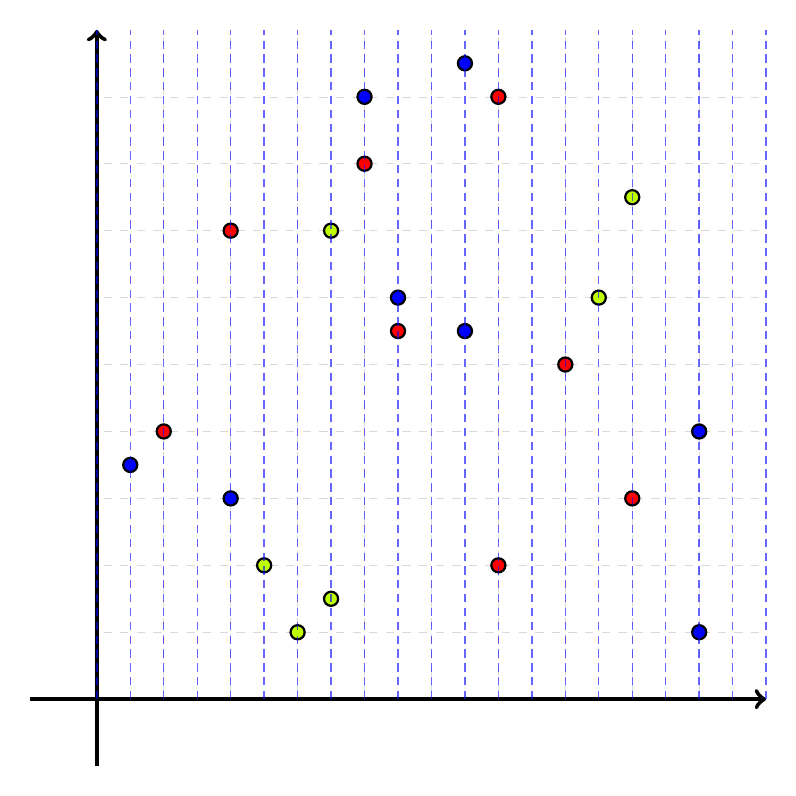
\begin{tikzpicture}[thick, scale=0.85]
%%%%% Axis %%%%%
\draw[help lines, color=gray!30, dashed] (-4.9,-4.9) grid (4.9,4.9);
\draw[->,ultra thick] (-6,-5)--(5,-5) ;
\draw[->,ultra thick] (-5,-6)--(-5,5) ;
%%%%% Blue Point %%%%%
\draw[fill=lime,draw=black] (2.5,1) circle (3pt);
\draw[fill=lime,draw=black] (-2,-4) circle (3pt);
\draw[fill=lime,draw=black] (3,2.5) circle (3pt);
\draw[fill=lime,draw=black] (-2.5,-3) circle (3pt);
\draw[fill=lime,draw=black] (-1.5,2) circle (3pt);
\draw[fill=lime,draw=black] (-1.5,-3.5) circle (3pt);

\draw[fill=red,draw=black] (-1,3) circle (3pt);
\draw[fill=red,draw=black] (1,-3) circle (3pt);
\draw[fill=red,draw=black] (-3,2) circle (3pt);
\draw[fill=red,draw=black] (2,0) circle (3pt);
\draw[fill=red,draw=black] (-0.5,0.5) circle (3pt);
\draw[fill=red,draw=black] (1,4) circle (3pt);
\draw[fill=red,draw=black] (-4,-1) circle (3pt);
\draw[fill=red,draw=black] (3,-2) circle (3pt);

\draw[fill=blue,draw=black] (0.5,4.5) circle (3pt);
\draw[fill=blue,draw=black] (-0.5,1) circle (3pt);
\draw[fill=blue,draw=black] (-4.5,-1.5) circle (3pt);
\draw[fill=blue,draw=black] (4,-4) circle (3pt);
\draw[fill=blue,draw=black] (0.5,0.5) circle (3pt);
\draw[fill=blue,draw=black] (-1,4) circle (3pt);
\draw[fill=blue,draw=black] (-3,-2) circle (3pt);
\draw[fill=blue,draw=black] (4,-1) circle (3pt);
\foreach \i in {-5,-4.5,...,4.5,5}{
\draw[densely dashed,color=blue,line width=0.5pt,opacity=0.6] (\i,-5)--(\i,5);
}
% \node at (0,-6.25) {$S_j$};
\end{tikzpicture}
\end{figure}
Note that $S_n$ is $k\times 1$-dimensional matrix of the number of points of each color in the plane.\par
\hspace{1\baselineskip} Defined $V$ by the $k$-dimension vector of the number of points of each color in left region of orthogonal partition.
\begin{figure}[H]
\centering
\begin{subfigure}{0.49\textwidth}
\centering
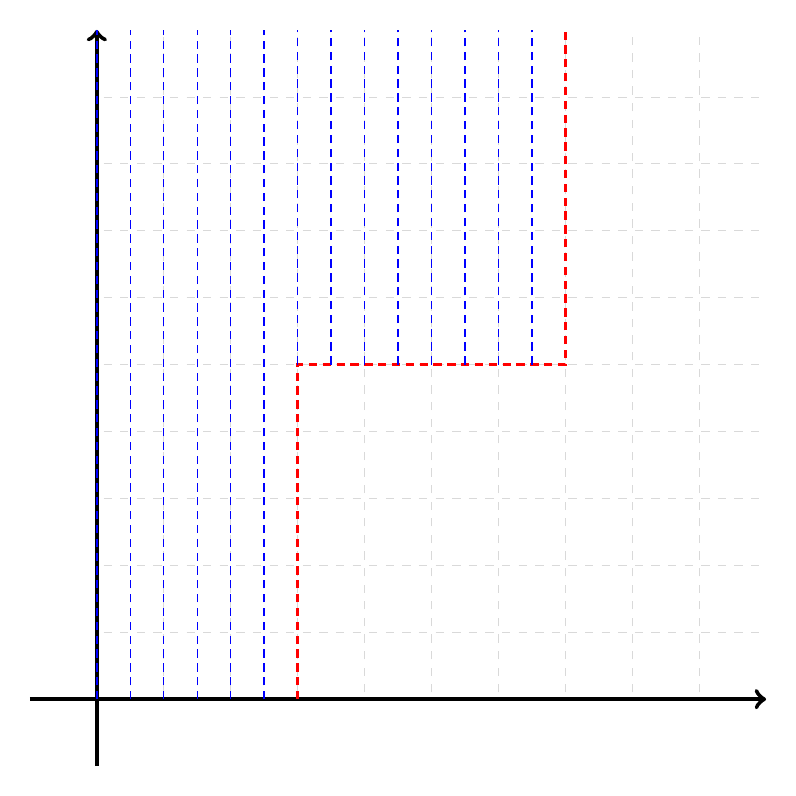
\begin{tikzpicture}[thick, scale=0.85]
%%%%% Axis %%%%%
\draw[help lines, color=gray!30, dashed] (-4.9,-4.9) grid (4.9,4.9);
\draw[->,ultra thick] (-6,-5)--(5,-5) ;
\draw[->,ultra thick] (-5,-6)--(-5,5) ;
\draw[densely dashed,color=red,line width=1pt,opacity=1](-2,-5)--(-2,0)--(2,0)--(2,5);
\foreach \i in {-5,-4.5,...,-3,-2.5}{
\draw[densely dashed,color=blue,line width=0.5pt,opacity=1] (\i,-5)--(\i,5);
}
\foreach \i in {-2,-1.5,...,1,1.5}{
\draw[densely dashed,color=blue,line width=0.5pt,opacity=1] (\i,0)--(\i,5);
}
% \node at (-5.5,0) {$\color{red!80!black}i_1$};
% \node at (-2,-5.5) {$\color{red!80!black}j_1$};
% \node at (2,-5.5) {$j$};
\end{tikzpicture}
\end{subfigure}
\begin{subfigure}{0.49\textwidth}
\centering
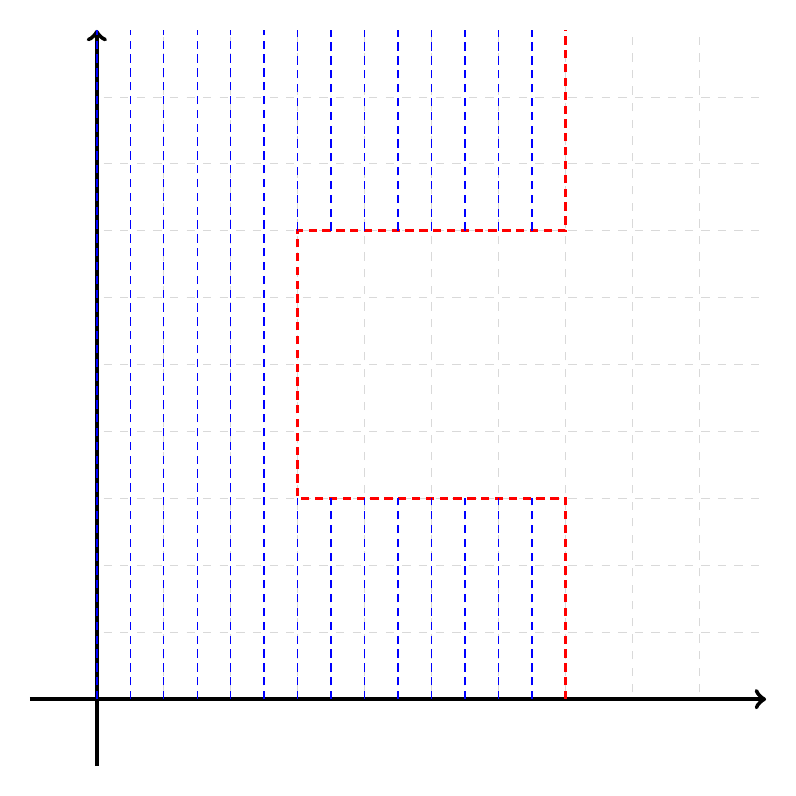
\begin{tikzpicture}[thick, scale=0.85]
%%%%% Axis %%%%%
\draw[help lines, color=gray!30, dashed] (-4.9,-4.9) grid (4.9,4.9);
\draw[->,ultra thick] (-6,-5)--(5,-5) ;
\draw[->,ultra thick] (-5,-6)--(-5,5) ;
\draw[densely dashed,color=red,line width=1pt,opacity=1] (2,-5)--(2,-2)--(-2,-2)--(-2,2)--(2,2)--(2,5);
% \node at (-5.5,-2) {$i_1$};
% \node at (-5.5,2) {$\color{red!80!black}i_2$};
% \node at (-2,-5.5) {$j_1$};
% \node at (2,-5.5) {$j$};
\foreach \i in {-5,-4.5,...,-3,-2.5}{
\draw[densely dashed,color=blue,line width=0.5pt,opacity=1] (\i,-5)--(\i,5);
}
\foreach \i in {-2,-1.5,...,1,1.5}{
\draw[densely dashed,color=blue,line width=0.5pt,opacity=1] (\i,-5)--(\i,-2);
\draw[densely dashed,color=blue,line width=0.5pt,opacity=1] (\i,2)--(\i,5);
}
\end{tikzpicture}
\end{subfigure}
\end{figure}
}
    
\posterbox[adjusted title= First Vertical Line]{name=first,column=2,span=1,below=abstract}{
Find a smallest $j\in\{0,\,1,\,\ldots,\,n\}$ satisfying 
$$\left\lfloor\dfrac{S_n}{2}\right\rfloor\le S_j$$

\begin{figure}[H]
    \centering
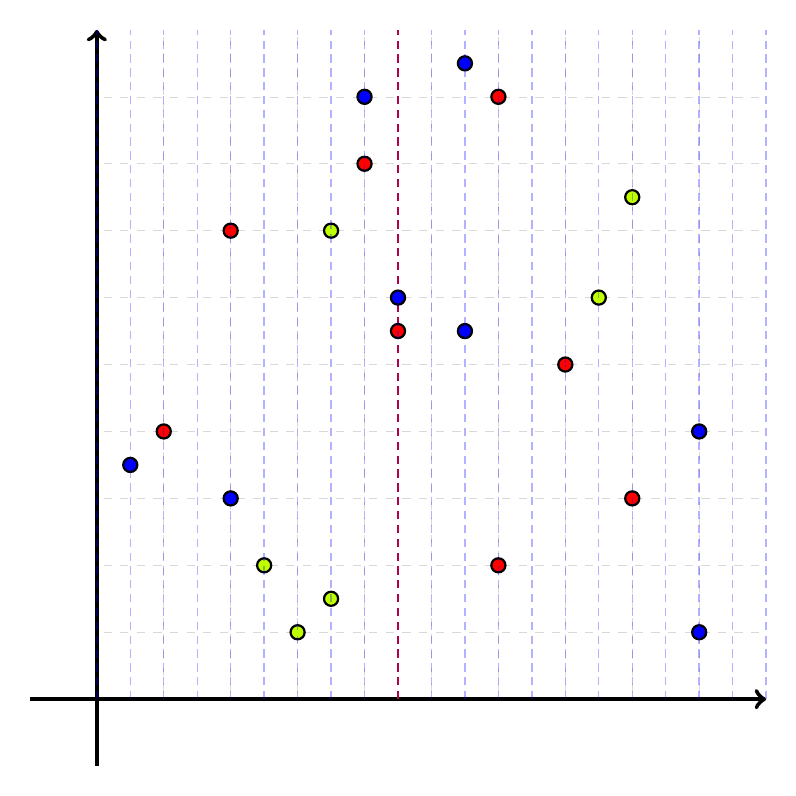
\begin{tikzpicture}[thick, scale=0.85]
%%%%% Axis %%%%%
\draw[help lines, color=gray!30, dashed] (-4.9,-4.9) grid (4.9,4.9);
\draw[->,ultra thick] (-6,-5)--(5,-5) ;
\draw[->,ultra thick] (-5,-6)--(-5,5) ;
\draw[densely dashed,color=red,line width=1pt,opacity=1] (-0.5,-5)--(-0.5,5);
%%%%% Point %%%%%
\draw[fill=lime,draw=black] (2.5,1) circle (3pt);
\draw[fill=lime,draw=black] (-2,-4) circle (3pt);
\draw[fill=lime,draw=black] (3,2.5) circle (3pt);
\draw[fill=lime,draw=black] (-2.5,-3) circle (3pt);
\draw[fill=lime,draw=black] (-1.5,2) circle (3pt);
\draw[fill=lime,draw=black] (-1.5,-3.5) circle (3pt);

\draw[fill=red,draw=black] (-1,3) circle (3pt);
\draw[fill=red,draw=black] (1,-3) circle (3pt);
\draw[fill=red,draw=black] (-3,2) circle (3pt);
\draw[fill=red,draw=black] (2,0) circle (3pt);
\draw[fill=red,draw=black] (-0.5,0.5) circle (3pt);
\draw[fill=red,draw=black] (1,4) circle (3pt);
\draw[fill=red,draw=black] (-4,-1) circle (3pt);
\draw[fill=red,draw=black] (3,-2) circle (3pt);

\draw[fill=blue,draw=black] (0.5,4.5) circle (3pt);
\draw[fill=blue,draw=black] (-0.5,1) circle (3pt);
\draw[fill=blue,draw=black] (-4.5,-1.5) circle (3pt);
\draw[fill=blue,draw=black] (4,-4) circle (3pt);
\draw[fill=blue,draw=black] (0.5,0.5) circle (3pt);
\draw[fill=blue,draw=black] (-1,4) circle (3pt);
\draw[fill=blue,draw=black] (-3,-2) circle (3pt);
\draw[fill=blue,draw=black] (4,-1) circle (3pt);
\foreach \i in {-5,-4.5,...,4.5,5}{
\draw[densely dashed,color=blue,line width=0.5pt,opacity=0.3] (\i,-5)--(\i,5);
}
\end{tikzpicture}
\end{figure}
It can be written in the form
\begin{equation*}
    V=S_j=\sum_{i=0}^{n}a_{ij}.
\end{equation*}
}
\posterbox[adjusted title=3 Line Segments]{name=3line,column=2,span=1,below=first}{
Given index $0<i_1<n$ and $0<j_1<n$ into $y-$axis and $x-$axis of first vertical line, respectively. The orthogonal partition when we added index $i_1,\,j_1$ as shown below.
\begin{figure}[H]
\centering
\begin{subfigure}{0.49\textwidth}
\centering
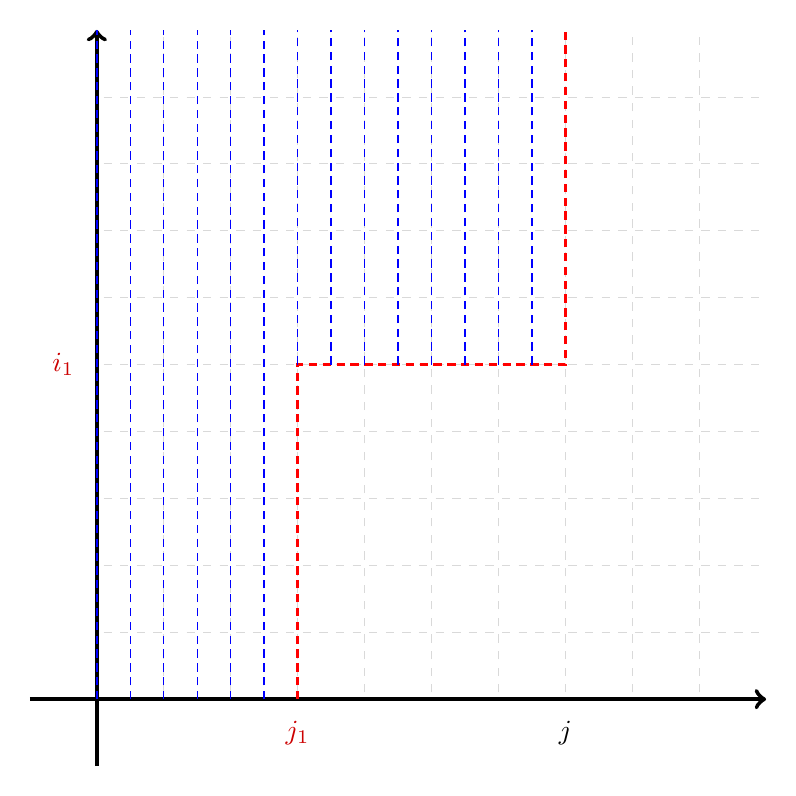
\begin{tikzpicture}[thick, scale=0.85]
%%%%% Axis %%%%%
\draw[help lines, color=gray!30, dashed] (-4.9,-4.9) grid (4.9,4.9);
\draw[->,ultra thick] (-6,-5)--(5,-5) ;
\draw[->,ultra thick] (-5,-6)--(-5,5) ;
\draw[densely dashed,color=red,line width=1pt,opacity=1](-2,-5)--(-2,0)--(2,0)--(2,5);
\foreach \i in {-5,-4.5,...,-3,-2.5}{
\draw[densely dashed,color=blue,line width=0.5pt,opacity=1] (\i,-5)--(\i,5);
}
\foreach \i in {-2,-1.5,...,1,1.5}{
\draw[densely dashed,color=blue,line width=0.5pt,opacity=1] (\i,0)--(\i,5);
}
\node at (-5.5,0) {$\color{red!80!black}i_1$};
\node at (-2,-5.5) {$\color{red!80!black}j_1$};
\node at (2,-5.5) {$j$};
\end{tikzpicture}
\end{subfigure}
\begin{subfigure}{0.49\textwidth}
\centering
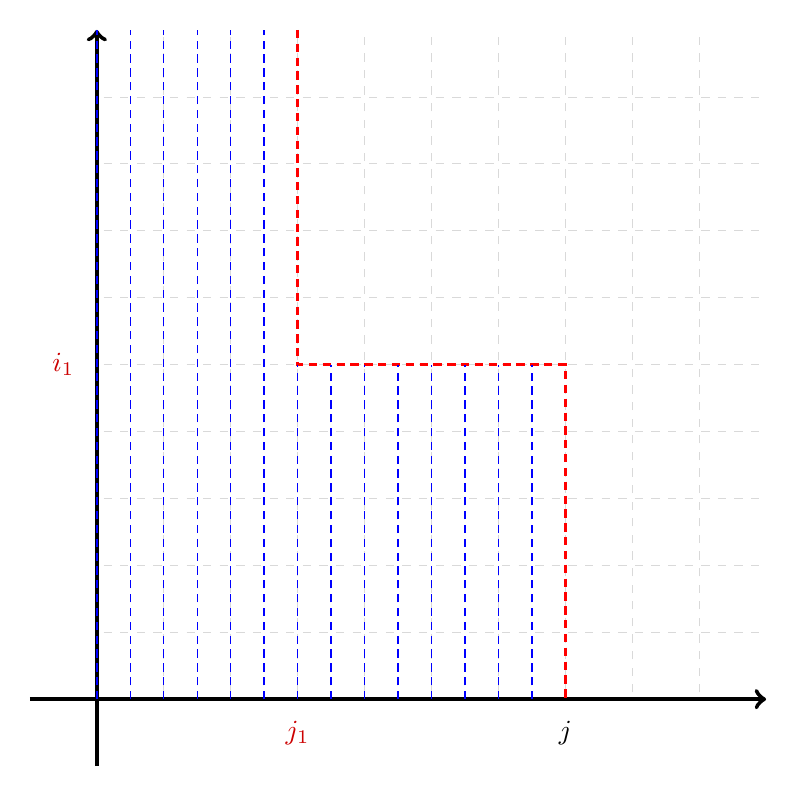
\begin{tikzpicture}[thick, scale=0.85]
%%%%% Axis %%%%%
\draw[help lines, color=gray!30, dashed] (-4.9,-4.9) grid (4.9,4.9);
\draw[->,ultra thick] (-6,-5)--(5,-5) ;
\draw[->,ultra thick] (-5,-6)--(-5,5) ;
\draw[densely dashed,color=red,line width=1pt,opacity=1](-2,5)--(-2,0)--(2,0)--(2,-5);
\foreach \i in {-5,-4.5,...,-3,-2.5}{
\draw[densely dashed,color=blue,line width=0.5pt,opacity=1] (\i,-5)--(\i,5);
}
\foreach \i in {-2,-1.5,...,1,1.5}{
\draw[densely dashed,color=blue,line width=0.5pt,opacity=1] (\i,-5)--(\i,0);
}
\node at (-5.5,0) {$\color{red!80!black}i_1$};
\node at (-2,-5.5) {$\color{red!80!black}j_1$};
\node at (2,-5.5) {$j$};

\end{tikzpicture}
\end{subfigure}
\end{figure}
It can be written in the form
\begin{equation*}
    V=\sum_{i=0}^{i_1}a_{ij}+\sum_{i=i_1}^{n}a_{ij_1}\quad\text{or}\quad V=\sum_{i=0}^{i_1}a_{ij_1} +\sum_{i=i_1}^{n}a_{ij},
\end{equation*}
where $0\le j_1\le j$.
}
\posterbox[adjusted title=Some Cases of 5 Line Segments]{name=5line,column=2,span=1,below=3line}{
Given an index $0<i_2<n$ into $y-$axis of three line segments. The orthogonal partition when we added index $i_1,\,j_1$ as shown below.

\begin{figure}[H]
\centering
\begin{subfigure}{0.49\textwidth}
\centering
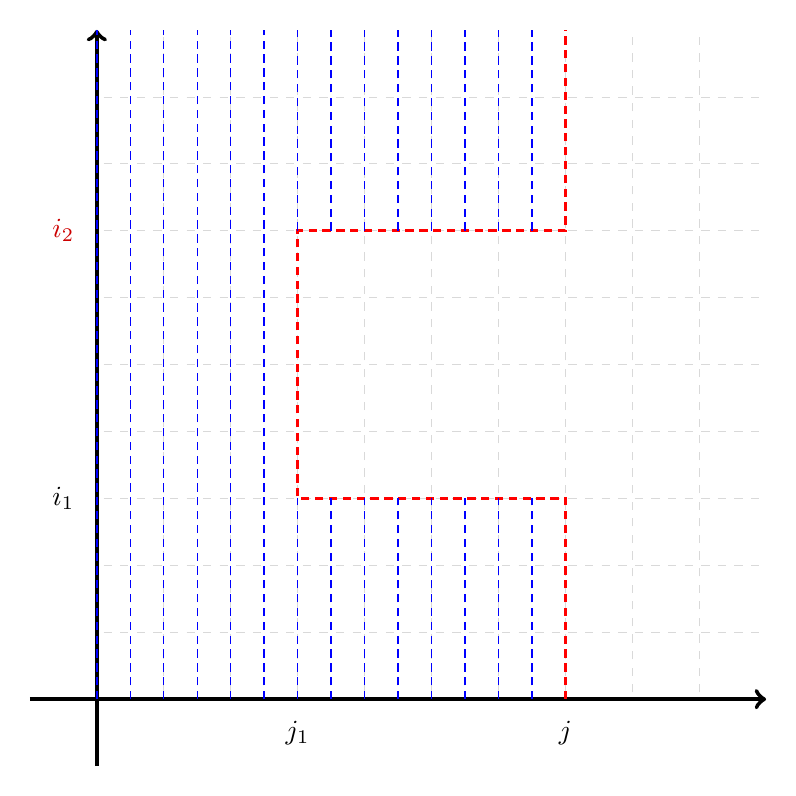
\begin{tikzpicture}[thick, scale=0.85]
%%%%% Axis %%%%%
\draw[help lines, color=gray!30, dashed] (-4.9,-4.9) grid (4.9,4.9);
\draw[->,ultra thick] (-6,-5)--(5,-5) ;
\draw[->,ultra thick] (-5,-6)--(-5,5) ;
\draw[densely dashed,color=red,line width=1pt,opacity=1] (2,-5)--(2,-2)--(-2,-2)--(-2,2)--(2,2)--(2,5);
\node at (-5.5,-2) {$i_1$};
\node at (-5.5,2) {$\color{red!80!black}i_2$};
\node at (-2,-5.5) {$j_1$};
\node at (2,-5.5) {$j$};
\foreach \i in {-5,-4.5,...,-3,-2.5}{
\draw[densely dashed,color=blue,line width=0.5pt,opacity=1] (\i,-5)--(\i,5);
}
\foreach \i in {-2,-1.5,...,1,1.5}{
\draw[densely dashed,color=blue,line width=0.5pt,opacity=1] (\i,-5)--(\i,-2);
\draw[densely dashed,color=blue,line width=0.5pt,opacity=1] (\i,2)--(\i,5);
}
\end{tikzpicture}
\end{subfigure}
\begin{subfigure}{0.49\textwidth}
\centering
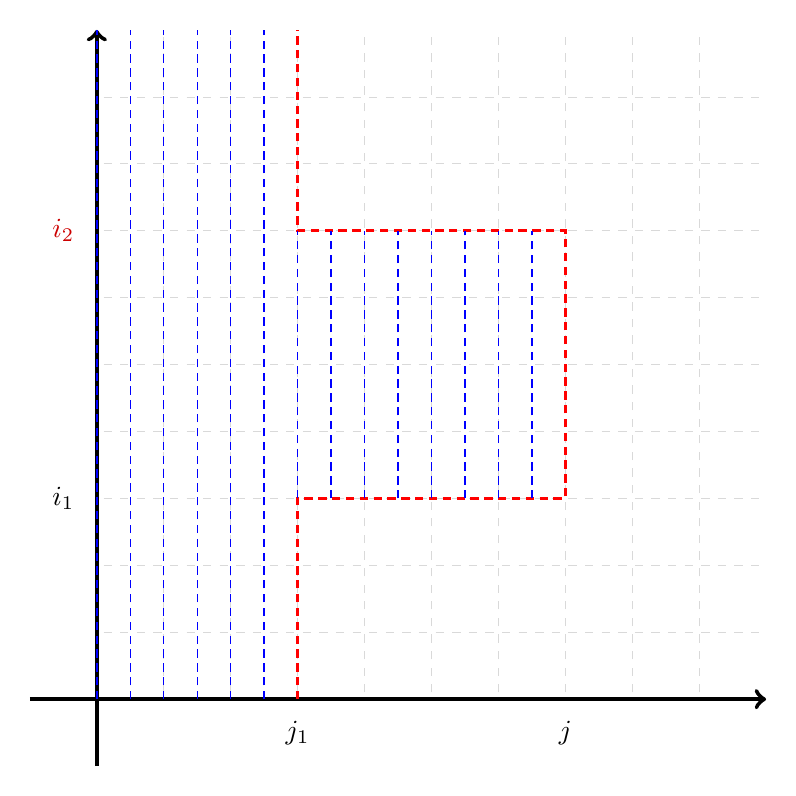
\begin{tikzpicture}[thick, scale=0.85]
%%%%% Axis %%%%%
\draw[help lines, color=gray!30, dashed] (-4.9,-4.9) grid (4.9,4.9);
\draw[->,ultra thick] (-6,-5)--(5,-5) ;
\draw[->,ultra thick] (-5,-6)--(-5,5) ;
\draw[densely dashed,color=red,line width=1pt,opacity=1](-2,-5)--(-2,-2)--(2,-2)--(2,2)--(-2,2)--(-2,5);
\node at (-5.5,-2) {$i_1$};
\node at (-5.5,2) {$\color{red!80!black}i_2$};
\node at (-2,-5.5) {$j_1$};
\node at (2,-5.5) {$j$};
\foreach \i in {-5,-4.5,...,-3,-2.5}{
\draw[densely dashed,color=blue,line width=0.5pt,opacity=1] (\i,-5)--(\i,5);
}
\foreach \i in {-2,-1.5,...,1,1.5}{
\draw[densely dashed,color=blue,line width=0.5pt,opacity=1] (\i,-2)--(\i,2);
}
\end{tikzpicture}
\end{subfigure}
\end{figure}
It can be written in the form
\begin{equation*}
V=\sum_{i=0}^{i_1}a_{ij}+\sum_{i=i_1}^{i_2}a_{ij_1}+\sum_{i=i_2}^{n}a_{ij},
\end{equation*}
or
\begin{equation*}
V=\sum_{i=0}^{i_1}a_{ij_1}+\sum_{i=i_1}^{i_2}a_{ij}+\sum_{i=i_2}^{n}a_{ij_1},
\end{equation*}
where $0\le j_1\le j$ and $0<i_1<i_2<n$.
}

\posterbox[adjusted title=Rotational Coordinate]{name=rotate, column=2,above=references}{
\hspace{1\baselineskip} For the algorithm above, we can swap between the coordinate $x,\,y$ and find orthogonal equipartitions with same iteration.
\begin{figure}[H]
\centering
\begin{subfigure}{0.49\textwidth}
\centering
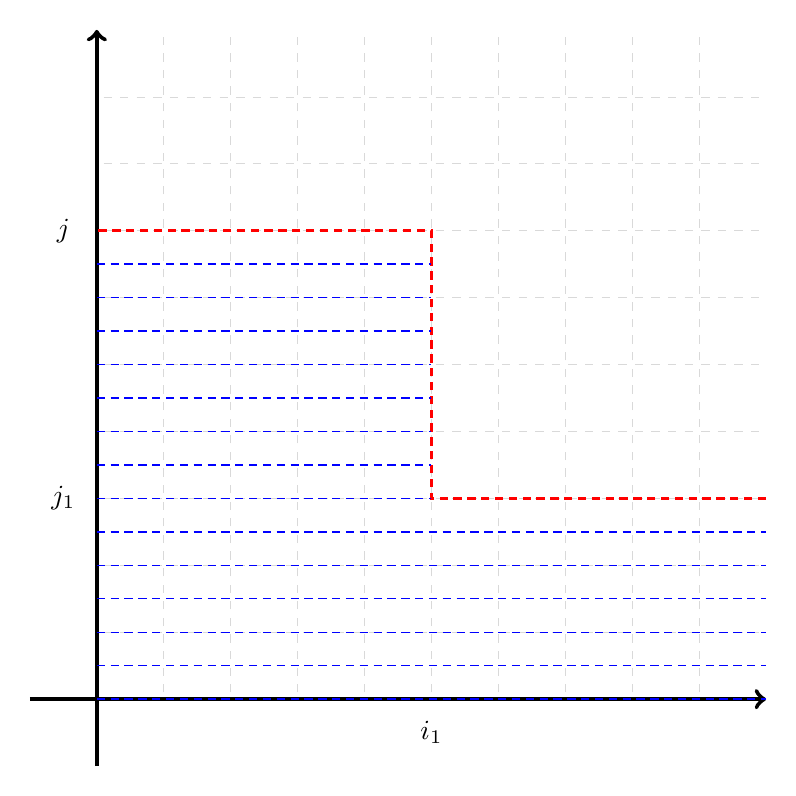
\begin{tikzpicture}[thick, scale=0.85]
%%%%% Axis %%%%%
\draw[help lines, color=gray!30, dashed] (-4.9,-4.9) grid (4.9,4.9);
\draw[->,ultra thick] (-6,-5)--(5,-5) ;
\draw[->,ultra thick] (-5,-6)--(-5,5) ;
\draw[densely dashed,color=red,line width=1pt,opacity=1](5,-2)--(0,-2)--(0,2)--(-5,2);
\foreach \i in {-5,-4.5,...,-3,-2.5}{
\draw[densely dashed,color=blue,line width=0.5pt,opacity=1] (-5,\i)--(5,\i);
}
\foreach \i in {-2,-1.5,...,1,1.5}{
\draw[densely dashed,color=blue,line width=0.5pt,opacity=1] (-5,\i)--(0,\i);
}
\node at (0,-5.5) {$i_1$};
\node at (-5.5,-2) {$j_1$};
\node at (-5.5,2) {$j$};

\end{tikzpicture}
\end{subfigure}
\begin{subfigure}{0.49\textwidth}
\centering
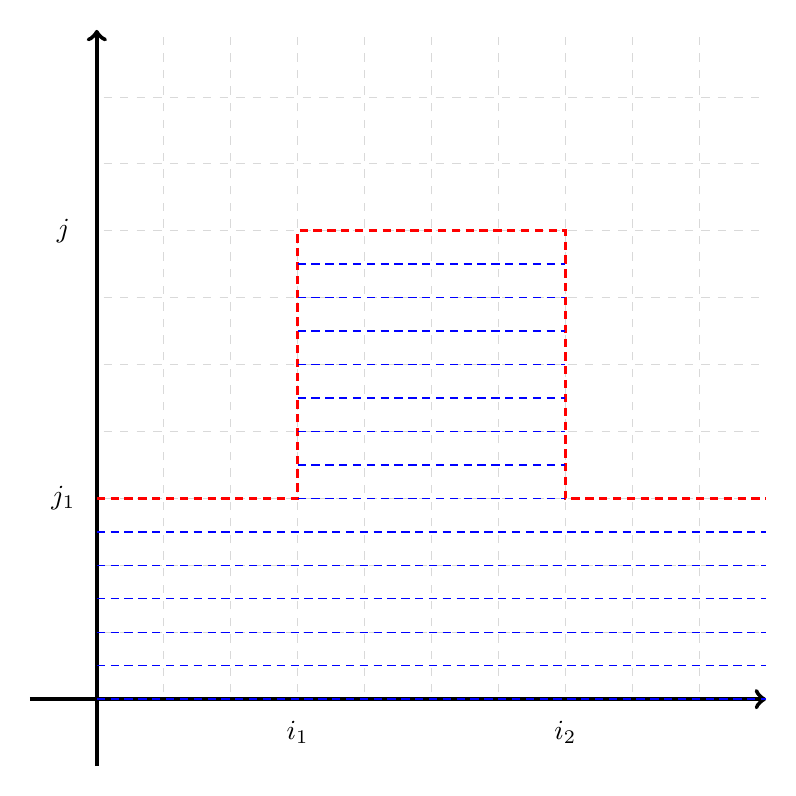
\begin{tikzpicture}[thick, scale=0.85]
%%%%% Axis %%%%%
\draw[help lines, color=gray!30, dashed] (-4.9,-4.9) grid (4.9,4.9);
\draw[->,ultra thick] (-6,-5)--(5,-5) ;
\draw[->,ultra thick] (-5,-6)--(-5,5) ;
\draw[densely dashed,color=red,line width=1pt,opacity=1](-5,-2)--(-2,-2)--(-2,2)--(2,2)--(2,-2)--(5,-2);
\node at (-5.5,-2) {$j_1$};
\node at (-5.5,2) {$j$};
\node at (-2,-5.5) {$i_1$};
\node at (2,-5.5) {$i_2$};
\foreach \i in {-5,-4.5,...,-3,-2.5}{
\draw[densely dashed,color=blue,line width=0.5pt,opacity=1] (-5,\i)--(5,\i);
}
\foreach \i in {-2,-1.5,...,1,1.5}{
\draw[densely dashed,color=blue,line width=0.5pt,opacity=1] (-2,\i)--(2,\i);
}
\end{tikzpicture}
\end{subfigure}

\end{figure}

}
\posterbox[adjusted title=Verify a Solution]{name=verify, column=2,between=5line and rotate}{
\hspace{1\baselineskip}     This orthogonal partition is a solution when $$\left|\dfrac{S_n}{2}-V\right|\le \dfrac{1}{2},$$
and it is a equitable when every element in matrix $S_n$ are even.
}

\posterbox[adjusted title=Results]{name=result, column=3,below=title}{
\hspace{1\baselineskip} The counterexample of 3 line segments for 3-color points.
\begin{figure}[H]
    \centering
    \includegraphics[width=0.71\linewidth]{False 3colors100x100_pic78.png}
\end{figure}
\hspace{1\baselineskip} The example of 5 line segments for 3-color points.
\begin{figure}[H]
    \centering
    \includegraphics[width=0.71\linewidth]{True 3colors100x100_pic15.png}
\end{figure}
\begin{figure}[H]
    \centering
    \includegraphics[width=0.71\linewidth]{True 3colors100x100_pic15.png}
\end{figure}
\begin{figure}[H]
    \centering
    \includegraphics[width=0.71\linewidth]{download (31).png}
\end{figure}
\hspace{1\baselineskip} An counterexample of some cases of 5 line segments for 4,\,5-color points, respectively.
\begin{figure}[H]
    \centering
    \includegraphics[width=0.71\linewidth]{False 4colors20x20_pic2094.png}
\end{figure}
\begin{figure}[H]
    \centering
    \includegraphics[width=0.71\linewidth]{False 5colors50x50_pic85.png}
\end{figure}

}
\posterbox[adjusted title=Conclusion]{name=conclusion, column=3,below=result}{
\hspace{1\baselineskip} In case 3-color points in general position have to use more than 3 line segments and it can find orthogonal equipartitions with 5 line segments for every sample from our generator. For $k$ greater than 3, we have counterexample for some cases of 5 line segments. However, It maybe partitioning by general case of 5 line segments as shown below.
\begin{figure}[H]
\centering
\begin{subfigure}{0.24\textwidth}
\centering
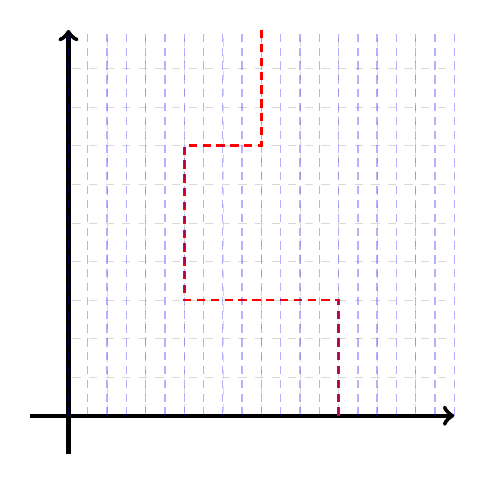
\begin{tikzpicture}[thick, scale=0.49]
%%%%% Axis %%%%%
\draw[help lines, color=gray!30, dashed] (-4.9,-4.9) grid (4.9,4.9);
\draw[->,ultra thick] (-6,-5)--(5,-5) ;
\draw[->,ultra thick] (-5,-6)--(-5,5) ;
\draw[densely dashed,color=red,line width=1pt,opacity=1] (2,-5)--(2,-2)--(-2,-2)--(-2,2)--(0,2)--(0,5);
\foreach \i in {-5,-4.5,...,4.5,5}{
\draw[densely dashed,color=blue,line width=0.5pt,opacity=0.3] (\i,-5)--(\i,5);
}
\end{tikzpicture}
\end{subfigure}
\begin{subfigure}{0.24\textwidth}
\centering
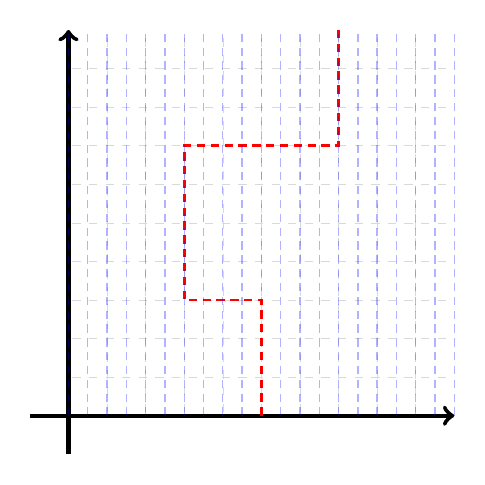
\begin{tikzpicture}[thick, scale=0.49]
%%%%% Axis %%%%%
\draw[help lines, color=gray!30, dashed] (-4.9,-4.9) grid (4.9,4.9);
\draw[->,ultra thick] (-6,-5)--(5,-5) ;
\draw[->,ultra thick] (-5,-6)--(-5,5) ;
\draw[densely dashed,color=red,line width=1pt,opacity=1] (2,5)--(2,2)--(-2,2)--(-2,-2)--(0,-2)--(0,-5);
\foreach \i in {-5,-4.5,...,4.5,5}{
\draw[densely dashed,color=blue,line width=0.5pt,opacity=0.3] (\i,-5)--(\i,5);
}
\end{tikzpicture}
\end{subfigure}
\begin{subfigure}{0.24\textwidth}
\centering
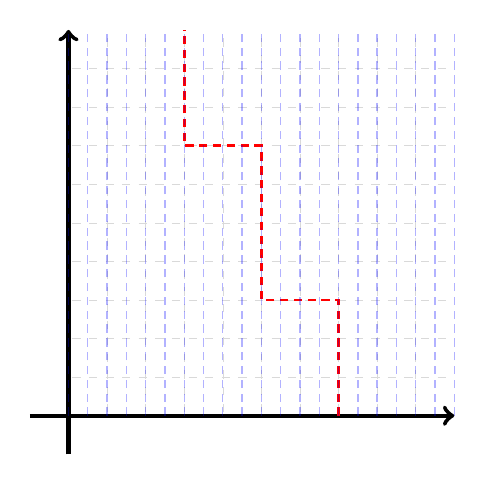
\begin{tikzpicture}[thick, scale=0.49]
%%%%% Axis %%%%%
\draw[help lines, color=gray!30, dashed] (-4.9,-4.9) grid (4.9,4.9);
\draw[->,ultra thick] (-6,-5)--(5,-5) ;
\draw[->,ultra thick] (-5,-6)--(-5,5) ;
\draw[densely dashed,color=red,line width=1pt,opacity=1] (2,-5)--(2,-2)--(0,-2)--(0,2)--(-2,2)--(-2,5);
\foreach \i in {-5,-4.5,...,4.5,5}{
\draw[densely dashed,color=blue,line width=0.5pt,opacity=0.3] (\i,-5)--(\i,5);
}
\end{tikzpicture}
\end{subfigure}
\begin{subfigure}{0.24\textwidth}
\centering
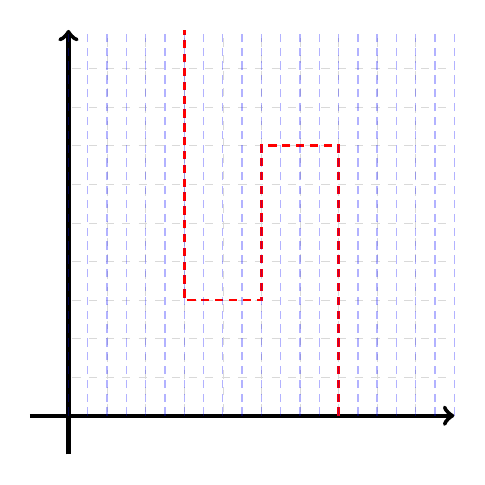
\begin{tikzpicture}[thick, scale=0.49]
%%%%% Axis %%%%%
\draw[help lines, color=gray!30, dashed] (-4.9,-4.9) grid (4.9,4.9);
\draw[->,ultra thick] (-6,-5)--(5,-5) ;
\draw[->,ultra thick] (-5,-6)--(-5,5) ;
\draw[densely dashed,color=red,line width=1pt,opacity=1] (2,-5)--(2,2)--(0,2)--(0,-2)--(-2,-2)--(-2,5);
\foreach \i in {-5,-4.5,...,4.5,5}{
\draw[densely dashed,color=blue,line width=0.5pt,opacity=0.3] (\i,-5)--(\i,5);
}
\end{tikzpicture}
\end{subfigure}
\begin{subfigure}{0.24\textwidth}
\centering
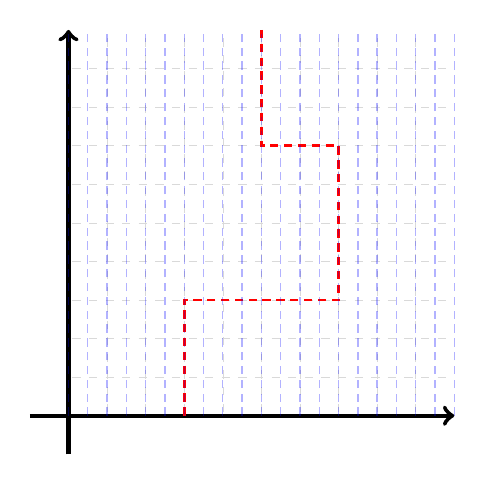
\begin{tikzpicture}[thick, scale=0.49]
%%%%% Axis %%%%%
\draw[help lines, color=gray!30, dashed] (-4.9,-4.9) grid (4.9,4.9);
\draw[->,ultra thick] (-6,-5)--(5,-5) ;
\draw[->,ultra thick] (-5,-6)--(-5,5) ;
\draw[densely dashed,color=red,line width=1pt,opacity=1] (0,5)--(0,2)--(2,2)--(2,-2)--(-2,-2)--(-2,-5);
\foreach \i in {-5,-4.5,...,4.5,5}{
\draw[densely dashed,color=blue,line width=0.5pt,opacity=0.3] (\i,-5)--(\i,5);
}
\end{tikzpicture}
\end{subfigure}
\begin{subfigure}{0.24\textwidth}
\centering
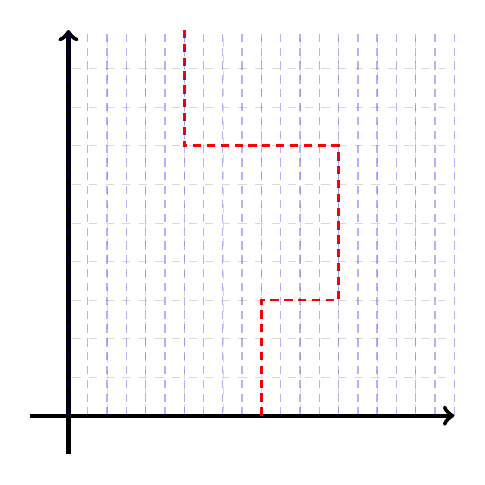
\begin{tikzpicture}[thick, scale=0.49]
%%%%% Axis %%%%%
\draw[help lines, color=gray!30, dashed] (-4.9,-4.9) grid (4.9,4.9);
\draw[->,ultra thick] (-6,-5)--(5,-5) ;
\draw[->,ultra thick] (-5,-6)--(-5,5) ;
\draw[densely dashed,color=red,line width=1pt,opacity=1] (-2,5)--(-2,2)--(2,2)--(2,-2)--(0,-2)--(0,-5);
\foreach \i in {-5,-4.5,...,4.5,5}{
\draw[densely dashed,color=blue,line width=0.5pt,opacity=0.3] (\i,-5)--(\i,5);
}
\end{tikzpicture}
\end{subfigure}
\begin{subfigure}{0.24\textwidth}
\centering
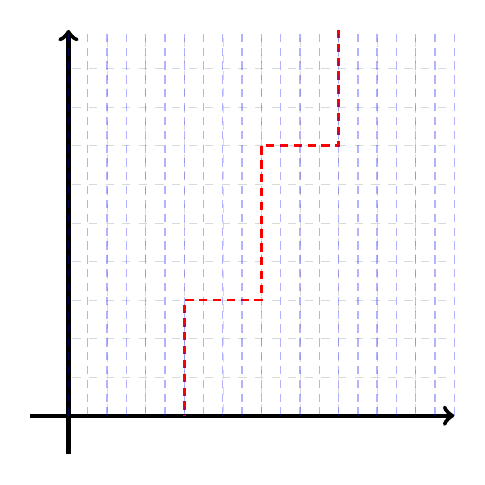
\begin{tikzpicture}[thick, scale=0.49]
%%%%% Axis %%%%%
\draw[help lines, color=gray!30, dashed] (-4.9,-4.9) grid (4.9,4.9);
\draw[->,ultra thick] (-6,-5)--(5,-5) ;
\draw[->,ultra thick] (-5,-6)--(-5,5) ;
\draw[densely dashed,color=red,line width=1pt,opacity=1] (2,5)--(2,2)--(0,2)--(0,-2)--(-2,-2)--(-2,-5);
\foreach \i in {-5,-4.5,...,4.5,5}{
\draw[densely dashed,color=blue,line width=0.5pt,opacity=0.3] (\i,-5)--(\i,5);
}
\end{tikzpicture}
\end{subfigure}
\begin{subfigure}{0.24\textwidth}
\centering
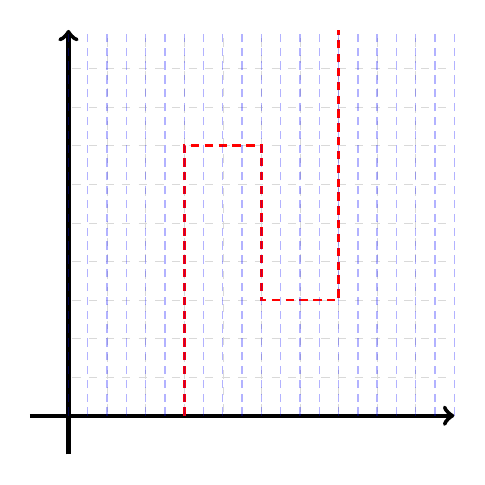
\begin{tikzpicture}[thick, scale=0.49]
%%%%% Axis %%%%%
\draw[help lines, color=gray!30, dashed] (-4.9,-4.9) grid (4.9,4.9);
\draw[->,ultra thick] (-6,-5)--(5,-5) ;
\draw[->,ultra thick] (-5,-6)--(-5,5) ;
\draw[densely dashed,color=red,line width=1pt,opacity=1] (-2,-5)--(-2,2)--(0,2)--(0,-2)--(2,-2)--(2,5);
\foreach \i in {-5,-4.5,...,4.5,5}{
\draw[densely dashed,color=blue,line width=0.5pt,opacity=0.3] (\i,-5)--(\i,5);
}
\end{tikzpicture}
\end{subfigure}
\end{figure}
In general case we add index $j_2,\,j_3$ for translation of vertical segments in previous some cases of 5 segments.
It can be written in the form
$$
    V=\sum_{i=0}^{i_1}a_{ij_1}+\sum_{i=i_1}^{i_2}a_{ij_2}+\sum_{i=i_2}^{n}a_{ij_3},$$
    \text{where $i_1\le i_2$, or}
    $$V=\sum_{i=0}^{i_1}a_{ij_1}-\sum_{i=i_1}^{i_2}a_{ij_2}+\sum_{i=i_2}^{n}a_{ij_3},
$$
where $i_1>i_2$.


}

\end{tcbposter}

\end{document}
